\documentclass[handout]{beamer}
\usetheme{Berlin}
\usecolortheme{seahorse}

\AtBeginSection[]{
  \begin{frame}
  \vfill
  \centering
  \begin{beamercolorbox}[sep=8pt,center,shadow=true,rounded=true]{title}
    \usebeamerfont{title}\insertsection\par%
  \end{beamercolorbox}
  \vfill
  \end{frame}
}

\usepackage{tikz}
\usepackage{ulem}
\usepackage{amsmath}
\usepackage{hyperref}

\renewcommand\iff\leftrightarrow
\newcommand{\RR}{\mathbb{R}}
\newcommand\del\nabla


\title{A gentle introduction to the calculus of variations}
\subtitle{(These slides: \href{http://bit.ly/intro-calc-var}{\color{magenta}bit.ly/intro-calc-var})}
\author{Spencer Bagley}
\institute{Westminster University \\
\href{https://sbagley.bsky.social}{\color{magenta}sbagley} on bluesky \\
\url{https://rhinopotamus.github.io}}
\date{}
\begin{document}
	\begin{frame}[plain]
	\maketitle
\end{frame}

\begin{frame}{Stuff we'll do here:}
\begin{columns}
\column{0.5\textwidth}
A vague outline of the talk:
\begin{itemize}
    \item A motivating problem
    \item An easier problem
    \item A general approach,
    \item applied to the first problem
\end{itemize}
\column{0.5\textwidth}
Math stuff we'll talk about:
\begin{itemize}
    \item Functionals
    \item Differentiation under the integral sign
    \item Integration by parts
    \item Some differential equations
    \item Lagrange multipliers
\end{itemize}
\end{columns}
\end{frame}

\section[Motivation]{A motivating problem}
{%
\usebackgroundtemplate{ %
\vbox to \paperheight{\vfil\hbox to \paperwidth{\hfil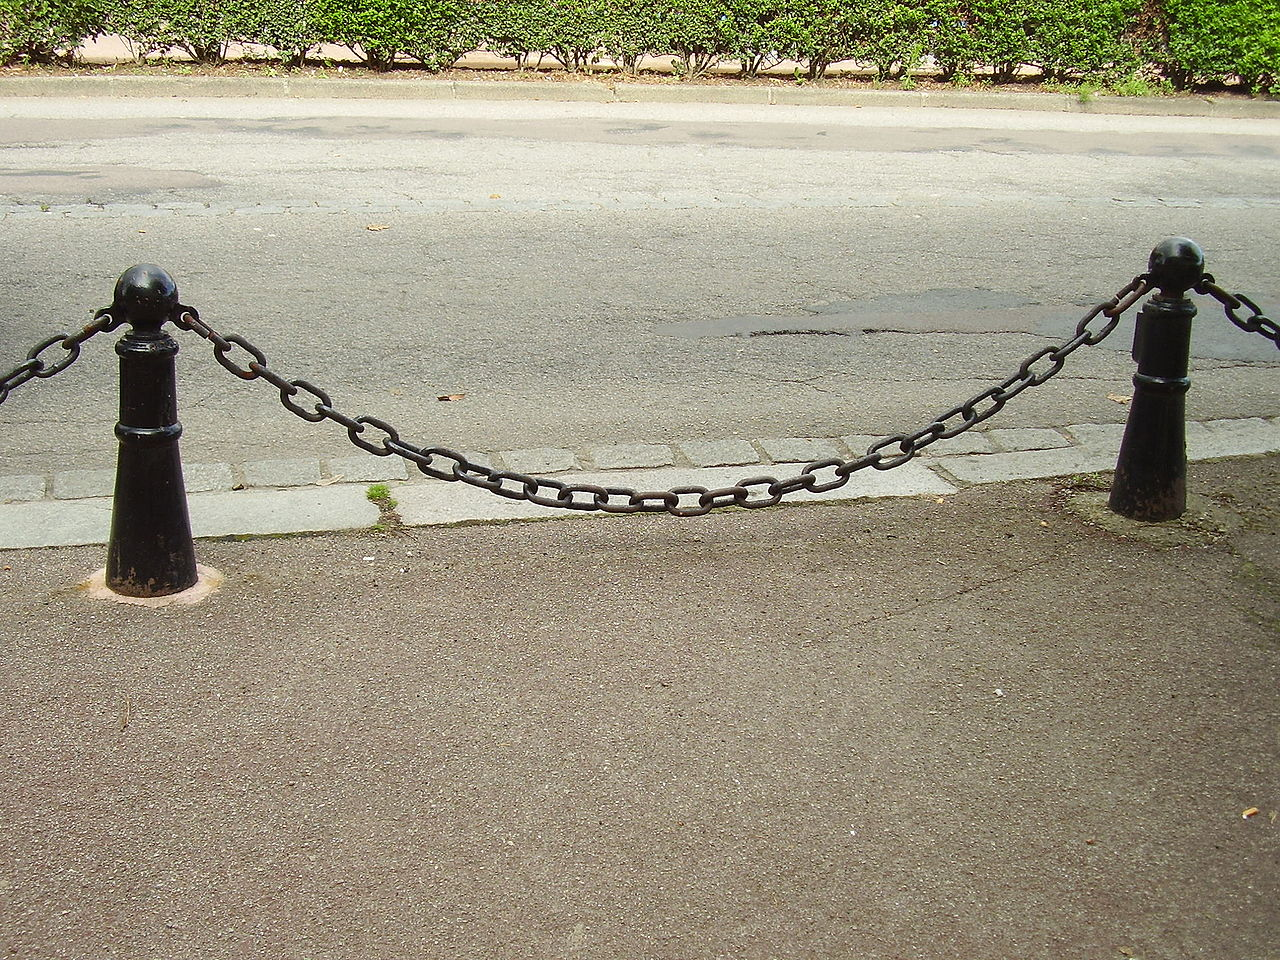
\includegraphics[width=0.8\textwidth]{catenary.jpg}\hfil}\vfil}
}
\begin{frame}[b]{The catenary}
\pause
\begin{block}{A motivating problem}
What function describes the shape taken by a hanging chain?
\end{block}
\end{frame}
}

\section[Functionals]{Functionals, variations, and ``wiggles''}

\begin{frame}{Functionals}
What is a function, anyway? \pause
\begin{itemize}
    \item Some kind of rule associating inputs with outputs \pause
    \item $f:\RR \to \RR$ \pause
\end{itemize}
A \alert{functional} is a function whose \alert{inputs} are functions \pause
\begin{itemize}
    \item $J: C^2 \to \RR$ \pause
    \item (or, y'know, whatever function space) \pause
    \item Most functionals we care about end up being definite integrals: 
    \[J[y] = \int_a^b f(x, y, y')\ dx\] \pause
\end{itemize}
(If I were naming this subject, I would call it ``the calculus of \alert{functionals},'' but nobody asked me)
\end{frame}

\begin{frame}{What if I want to minimize a functional?}
We want to take some kind of derivative\pause
\begin{itemize}
    \item (because derivatives are a nice way to handle extrema) \pause
\end{itemize}
\begin{block}{Definition (kinda)}
The \alert{derivative} is a device that measures \\
the effect on the output \hfill $dy$ \\
of small changes in the input. \hfill $dx$
\end{block} \pause
So how should we deal with this for functionals, where the inputs are themselves functions?

\end{frame}

\begin{frame}{Variations and ``wiggles''}
A \alert{variation} is a function $\eta(x)$ who is: \pause
\begin{itemize}
    \item \alert{not too wild}: piecewise $C^2$ or maybe even piecewise $C^1$ \pause
    \item \alert{zero at endpoints}: $\eta(x_1) = \eta(x_2) = 0$ \pause
\end{itemize}
A \alert{``wiggle''} is the result of adding some \alert{a}mount of variation to a base function: \pause
\begin{itemize}
    \item $w(x) = y(x) + \alert{a}\ \eta(x)$ \pause
    \item ``A one-parameter family of curves'' that includes original $y(x)$ (when $a=0$)
\end{itemize}\pause
\begin{beamercolorbox}[sep=4pt,shadow=true,rounded=true]{title}
    ``Wiggles'' seem like a good way to capture the idea of ``small changes to inputs'' in the context of functionals.
\end{beamercolorbox}

\end{frame}

\begin{frame}{Derivatives of functionals}
    Instead of feeding the functional $J$ the original function $y$, let's feed it a wiggle $w=y + a\eta$:
    \[J[w] = J[y+a\eta] = \int_{x_1}^{x_2}f(x, y+a\eta, y'+a\eta')\ dx\]
    
    \pause
    This is truly a \alert{function} of $a$! \pause
    \[J_y(a) = \int_{x_1}^{x_2}f(x, y+a\eta, y'+a\eta')\ dx\] \pause
    I can just regular-calculus-differentiate w.r.t. $a$! \pause (I hope)
\end{frame}

\begin{frame}{Our strategy}
\begin{itemize}
    \item Write down a functional: $J[y]=\displaystyle\int_{x_1}^{x_2}f(x, y, y')\ dx$
    \item Construct a ``wiggle'' by adding ``variation:'' $w(x) = y(x) + a\cdot\eta(x)$
    \item Apply the functional to the wiggle: $J(a) = J[y+a\eta] =\displaystyle\int_{x_1}^{x_2}f(x, y+a\eta, y'+a\eta')\ dx$
    \item Take some kind of derivative: $\frac{d}{da}J(a)$
    \item Assume $y$ (corresponding to $a=0$) is a minimizer: 
    \begin{itemize} \item Assert $J'(0)=0$ \end{itemize}
    \item Try to conclude something interesting about $y$
\end{itemize}
\end{frame}

%%%%%%%%%%%%%%%%%%%%%%%%%%%%%%%%%%%%%%%%%%%%%%%%%%%%%%%%%%%%%%%%%%%%%%%%%%%%%%%%%%%%%
\section*{Derivatives}
\begin{frame}
    \begin{beamercolorbox}[sep=8pt,center,shadow=true,rounded=true]{title}
    \usebeamerfont{title} ``Some kind of derivative,'' eh?
\end{beamercolorbox}
Let's think a bit harder about how this, theoretically, just-plain-calculus derivative $\frac{d}{da} J(a)$ actually works.
\end{frame}


\begin{frame}{Differentiating under the integral sign}
    \[\dfrac{d}{da} J(a) = \dfrac{d}{da} \left[\int_{x_1}^{x_2}f(x, y+a\eta, y'+a\eta')\ dx\right]\] \pause
    Oh no, all of my $a$'s are inside this integral, whatever shallst I do \pause
\begin{block}{Leibniz integral rule {\tiny (sometimes this is called Feynman's integral trick but he's kind of a jerk)}}
As long as the integrand is continuous, 
\[\dfrac{d}{da}\left[\displaystyle\int_{x_1}^{x_2}g(x,a)\ dx\right] = \displaystyle\int_{x_1}^{x_2}\left[\dfrac{\partial}{\partial a} g(x,a)\right]\ dx\]
(\alert{Note:} $d/da$ outside becomes $\partial/\partial a$ inside)
\end{block}\pause
\begin{itemize}
    \item This is basically Fubini's theorem \pause and/or Clairault's theorem
\end{itemize}
\end{frame}

\begin{frame}{Okay, so,}
    \begin{align*}
        \dfrac{d}{da} J(a) &= \dfrac{d}{da} \left[\int_{x_1}^{x_2}f(x, y+a\eta, y'+a\eta')\ dx\right] \\ \pause
        &= \int_{x_1}^{x_2} \left[\dfrac{\partial}{\partial a} f(x, y+a\eta, y'+a\eta') \right]\ dx \pause 
        \intertext{or in other words}
        &= \int_{x_1}^{x_2} \left[\dfrac{\partial}{\partial a} f(x, w, w') \right]\ dx
    \end{align*}
    I guess let's zoom in on this integrand $\dfrac{\partial f}{\partial a}$.
\end{frame}

\begin{frame}{Chain rule: How does $f$ depend on $a$?}
\begin{columns}
\begin{column}{0.4\textwidth}
\begin{center}
    \begin{tikzpicture}
    \node {$f$}
        child { node {$x$} }
        child { node {$w$}
            child { node {$a$} } }
        child { node {$w'$}
            child {node {$a$} } };
    \end{tikzpicture}
    \end{center} \pause
    
    \[\dfrac{\partial f}{\partial a} = 
      \dfrac{\partial f}{\partial w}
      \dfrac{\partial w}{\partial a} +
      \dfrac{\partial f}{\partial w'}
      \dfrac{\partial w'}{\partial a} \] \pause
\end{column}
\vrule{}
\begin{column}{0.6\textwidth}
\begin{itemize}
\item Well, $\dfrac{\partial w}{\partial a} = \eta$, and $\dfrac{\partial w'}{\partial a} = \eta'$ \pause

\item so $ \dfrac{\partial f}{\partial a} = 
      \dfrac{\partial f}{\partial w}
      \cdot \eta +
      \dfrac{\partial f}{\partial w'}
      \cdot \eta' $ \pause
\item and we're interested in $a=0$ where $w=y+0\eta$ \pause
\item Thus,
\end{itemize}

\[ \left.\dfrac{\partial f}{\partial a} \right|_{a=0} = 
      \dfrac{\partial f}{\partial y}
      \cdot \eta +
      \dfrac{\partial f}{\partial y'}
      \cdot \eta' \]
\end{column}
\end{columns}
\end{frame}

\begin{frame}{Zooming back out}
    \begin{align*}
        \dfrac{d}{da} J(a) &= \dfrac{d}{da} \left[\int_{x_1}^{x_2}f(x, y+a\eta, y'+a\eta')\ dx\right] \\
        &= \int_{x_1}^{x_2} \left[\dfrac{\partial}{\partial a} f(x, w, w') \right]\ dx \\ \pause
        &= \int_{x_1}^{x_2} \left[
            \dfrac{\partial f}{\partial w}  \cdot \eta +
            \dfrac{\partial f}{\partial w'} \cdot \eta'
            \right]\ dx \\ \pause
        \left. \dfrac{d}{da} J(a) \right|_{a=0} &= 
            \int_{x_1}^{x_2} \dfrac{\partial f}{\partial y} \cdot \eta +
            \dfrac{\partial f}{\partial y'} \cdot \eta' \ dx 
    \end{align*}
    We're then asserting that this last integral is zero.
\end{frame}

\begin{frame}{Observations:}
    \[0 = \left.\dfrac{d}{da} J(a) \right|_{a=0} = 
            \int_{x_1}^{x_2} \dfrac{\partial f}{\partial y} \cdot \eta +
            \dfrac{\partial f}{\partial y'} \cdot \eta' \ dx\] \pause
    \begin{itemize}
        \item These two summands look suspiciously similar. \pause
        \item In the first, we have something multiplied against $\eta$; \pause
        \item in the second, something multiplied against $\eta'$. \pause
        \item Maybe we can exploit this structure.
    \end{itemize}
\end{frame}
%%%%%%%%%%%%%%%%%%%%%%%%%%%%%%%%%%%%%%%%%%%%%%%%%%%%%%%%%%%%%%%%%%%%%%%%%%%%%%%%%%%%%
\section[FLCOV]{The Fundamental Lemma \\ of the Calculus of Variations}

\begin{frame}{Lemma time}
    \begin{alertblock}{The Fundamental Lemma of the Calculus of Variations (!!!)}
    Suppose $m(x)$ is continuous. If $\int_{x_1}^{x_2}m(x) \cdot \eta(x)\ dx = 0$ for \alert{all} variations $\eta$, then $m(x) \equiv 0$.
    \end{alertblock} \pause
    Observations: \pause
    \begin{itemize}
        \item This is truly just the $L_2$ inner product $\langle m, \eta \rangle$ \pause
        \item So what this says is, the only thing that's orthogonal to every variation is the zero function \pause
        \item (This restatement makes it more believable to me)
    \end{itemize}
\end{frame}

\begin{frame}
\begin{proof}
Suppose not: \pause say WLOG that $m(x^*) > 0$. \pause Since $m$ is continuous, there exists an interval $[c,d]$ around $x^*$ on which $m(x) > 0$. \\\pause
Let $\eta(x) = 
\begin{cases} 
    0 & x\not\in[c,d] \\
    (x-c)(d-x) & x \in[c,d]
\end{cases}
$. \pause \quad $\eta$ is a variation. \pause

\[\arraycolsep=1pt
\begin{array}{cccc}
0 &= \int_{x_1}^{x_2}m(x) \cdot \eta(x)\ dx & & \\[5pt] \pause
  &= \int_{x_1}^{c}m(x) \cdot \eta(x)\ dx &
      + \int_{c}^{d}m(x) \cdot \eta(x)\ dx &
      + \int_{d}^{x_2}m(x) \cdot \eta(x)\ dx  \\[5pt] \pause
  & 0 & >0 & 0
\end{array}
\]\pause
So we have $0 > 0$, and we've reached our \textbf{contradiction.}
\end{proof}
\end{frame}

\iffalse
\begin{frame}{We need a lemma}
    \begin{alertblock}{The Fundamental Lemma of the Calculus of Variations (!!!)}
    Suppose $m(x)$ is continuous. If $\int_{x_1}^{x_2}m(x) \cdot \eta(x)\ dx = 0$ for \alert{all} variations $\eta$, then $m(x) \equiv 0$.
    \end{alertblock}
    \begin{block}{Corollary}
    Suppose $M(x)$ is continuous. If $\int_{x_1}^{x_2}M(x) \cdot \eta\alert{'}(x)\ dx = 0$ for \alert{all} variations $\eta$, then $M(x)$ is a constant function.
    \end{block} \pause
\begin{proof}
Integrate by parts!
\end{proof}
\end{frame}
\fi

%%%%%%%%%%%%%%%%%%%%%%%%%%%%%%%%%%%%%%%%%%%%%%%%%%%%%%%%%%%%%%%%%%%%%%%%%%%%%%%%%%%%%
\section[Euler-Lagrange]{The Euler-Lagrange equation}

\begin{frame}{Reminder of our strategy}
\begin{itemize}
    \item Write down a functional: $J[y]=\displaystyle\int_{x_1}^{x_2}f(x, y, y')\ dx$
    \item Construct a ``wiggle'' by adding ``variation:'' $w(x) = y(x) + a\cdot\eta(x)$
    \item Apply the functional to the wiggle: $J(a) = J[y+a\eta] =\displaystyle\int_{x_1}^{x_2}f(x, y+a\eta, y'+a\eta')\ dx$
    \item Take some kind of derivative: $\frac{d}{da}J(a)$
    \item Assume $y$ (corresponding to $a=0$) is a minimizer: 
    \begin{itemize} \item Assert $J'(0)=0$ \alert{$\leftarrow$ We are here}
    \end{itemize}
    \item Try to conclude something interesting about $y$
\end{itemize}
\end{frame}

\begin{frame}{Ready for some integration by parts?}
    \begin{alignat*}{2}
        \int_{x_1}^{x_2} \dfrac{\partial f}{\partial a}\, dx &=
        \int_{x_1}^{x_2} 
      \dfrac{\partial f}{\partial y}
      \cdot \eta && +
      {\color{blue}\dfrac{\partial f}{\partial y'} \cdot \eta'} 
      \ dx \\
      & && \color{blue}\begin{array}{ll}
\onslide<4->{\phantom{d}u = \frac{\partial f}{\partial y'}} & 
\onslide<3->{\phantom{d}v = \eta} \\
\onslide<5->{du = \frac{d}{dx}\left(\frac{\partial f}{\partial y'}\right)dx      } & 
\onslide<2->{dv = \eta'\ dx }
\end{array} \\
& && \onslide<6->{\color{blue} \left[\tfrac{\partial f}{\partial y'}\cdot \eta \right|_{x_1}^{x_2} - \int_{x_1}^{x_2}\eta\cdot \frac{d}{dx}\left(\frac{\partial f}{\partial y'}\right)dx} \\
& \onslide<7->{= \int_{x_1}^{x_2} \dfrac{\partial f}{\partial y} \cdot \eta 
&& - \frac{d}{dx}\left(\frac{\partial f}{\partial y'}\right)\cdot \eta\ dx} \\
& \onslide<8->{=\int_{x_1}^{x_2} 
{\color{red} \left(
\dfrac{\partial f}{\partial y} \right.}
&& {\color{red} \left. - \frac{d}{dx}\left(\frac{\partial f}{\partial y'}\right) \right)} \cdot \eta\ dx} 
\onslide<9->{= 0} \onslide<10->{\qquad \color{red}{\text{FLCOV!!!}}}
    \end{alignat*}
\end{frame}

\begin{frame}{Conclude something interesting about $y$}
\begin{block}{Euler-Lagrange equation}
If $y$ is a minimizer for the functional $J[y] = \displaystyle\int_{x_1}^{x_2} f(x, y, y')\ dx$, then $y$ satisfies the equation

\[\dfrac{\partial f}{\partial y} - \dfrac{d}{dx}\left(\dfrac{\partial f}{\partial y'}\right) = 0. \quad\left(
\text{Or, }
\frac{\partial f}{\partial y} = \frac{d}{dx}\left(\frac{\partial f}{\partial y'}\right).\right)\]
\end{block}
\end{frame}

\begin{frame}{Toward a special case}
This $\frac{d}{dx}$ business is weird. Let's think about $\frac{df}{dx}$.
\begin{columns}
\begin{column}{0.3\textwidth}
\onslide<2->{
\begin{center}
    \begin{tikzpicture}
        \node {$f$}
            child {node {$x$} }
            child {node {$y$}
                child {node {$x$}}}
            child { node {$y'$}
                child { node {$x$}} };
    \end{tikzpicture} \pause
\end{center}
}
\end{column}
\begin{column}{0.7\textwidth}
\begin{align*}
    \onslide<3->{\frac{df}{dx} &= \frac{\partial f}{\partial y} \cdot 
                     \frac{dy}{dx} + 
                     \frac{\partial f}{\partial y'} \cdot
                     \frac{dy'}{dx} + 
                     \frac{\partial f}{\partial x}} \\
\onslide<4->{&= \frac{d}{dx}\left(\frac{\partial f}{\partial y'}\right) 
   \cdot y' +              
   \frac{\partial f}{\partial y'} 
   \cdot \frac{d}{dx}(y') + 
   \frac{\partial f}{\partial x}}
\onslide<5->{\intertext{Apply the product rule backward!}}
\onslide<6->{&= \frac{d}{dx}\left(\frac{\partial f}{\partial y'}
                     \cdot y'\right) + 
   \frac{\partial f}{\partial x}}\\
\onslide<7->{\frac{df}{dx} &- \frac{d}{dx}\left(\frac{\partial f}{\partial y'}
                     \cdot y'\right) = \frac{\partial f}{\partial x}}
\end{align*}
\end{column}
\end{columns}
\end{frame}

\begin{frame}{Toward a special case}
    So, suppose that $\dfrac{\partial f}{\partial x} = 0.$ \pause
\onslide<2->{
    \begin{itemize}
        \item In other words, the integrand of the functional doesn't depend explicitly on $x$
        \item (This happens frequently because many situations we'd care about are autonomous slash time-invariant)
    \end{itemize}
}
\onslide<3->{Then:}
    \begin{align*}
        \onslide<3->{\frac{df}{dx} - \frac{d}{dx}\left(\frac{\partial f}{\partial y'} \cdot y'\right) &= \frac{\partial f}{\partial x} = 0\\}
        \onslide<4->{\frac{d}{dx}\left(f - \dfrac{\partial f}{\partial y'} \cdot y' \right) &= 0 \\}
        \onslide<5->{ f - \dfrac{\partial f}{\partial y'} \cdot y' &= C}
    \end{align*}
\end{frame}

\begin{frame}{Conclude something interesting about $y$, part deux}
\begin{block}{Euler-Lagrange equation}
If $y$ is a minimizer for the functional $J[y] = \int_{x_1}^{x_2} f(x, y, y')\ dx$, then $y$ satisfies the equation

\[\dfrac{\partial f}{\partial y} - \dfrac{d}{dx}\left(\dfrac{\partial f}{\partial y'}\right) = 0. \quad\left(
\text{Or, }
\frac{\partial f}{\partial y} = \frac{d}{dx}\left(\frac{\partial f}{\partial y'}\right).\right)\]
\end{block}

\begin{alertblock}{Special case: Beltrami identity}
If $\frac{\partial f}{\partial x} = 0$, then $y$ satisfies the equation
\[f - \dfrac{\partial f}{\partial y'} \cdot y' = C.\]
\end{alertblock}
\end{frame}


%%%%%%%%%%%%%%%%%%%%%%%%%%%%%%%%%%%%%%%%%%%%%%%%%%%%%%%%%%%%%%%%%%%%%%%%%%%%%%%%%%%%%
\section{Some examples}
\subsection{Arc length}

\begin{frame}{Example: arc length}
(Fun toy: \href{https://www.wolframalpha.com/input/?i=arc+length}{\color{magenta}Wolfram Alpha ``arc length''}) \pause

Put in a function, get out its length \pause (between two $x$-values) \pause

Let's do a little calculus: \pause \alert{slice-approximate-integrate}

\begin{columns}
\column{0.35\linewidth}
\begin{figure}
    \begin{overprint}
    \onslide<6|handout:0>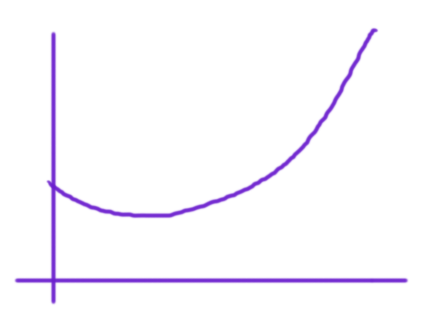
\includegraphics[width=\textwidth]{arclength-1.png}
    \onslide<7|handout:0>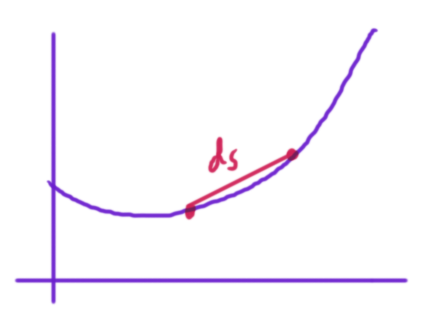
\includegraphics[width=\textwidth]{arclength-2.png}
    \onslide<8->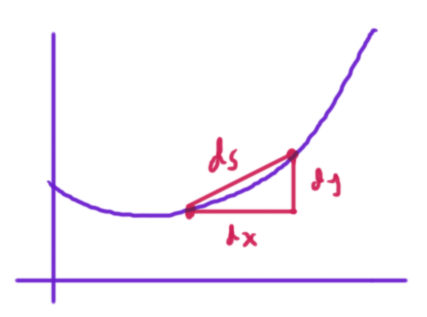
\includegraphics[width=\textwidth]{arclength-3.png}
    \end{overprint}
\end{figure}
\column{0.6\linewidth}
\begin{align*}
    \onslide<9->{ds^2 &= dx^2 + dy^2\\}
    \onslide<10->{&=\left(1+\frac{dy^2}{dx^2}\right)dx^2\\}
    \onslide<11->{ds &= \sqrt{1+\left(\frac{dy}{dx}\right)^2}dx\\}
    \onslide<12->{ &= \sqrt{1+(y')^2}\ dx}
\end{align*}

\end{columns}

\end{frame}

\begin{frame}{Example: Arc length}
Cool, so $J[y] = \int ds = 
\displaystyle\int_{x_1}^{x_2}\sqrt{1+(y')^2}\ dx$ \pause
$ = \displaystyle\int_{x_1}^{x_2}f(x, y, y')\ dx $
Some notes: \pause
\begin{itemize}
    \item \alert{Most} functionals we care about end up being definite integrals\pause
    \item \alert{Many} functionals we care about don't depend explicitly on $x$ \pause
\end{itemize}
\begin{block}{An easier problem}
What function connecting two given points $(x_1, y_1)$ and $(x_2, y_2)$ has the \alert{minimal} arc length? \pause
\alert{Note:} You can at this point just apply the Beltrami identity, but let's have some fun.
\end{block}
\end{frame}



\begin{frame}{The arc length of a wiggle}
\href{https://www.desmos.com/calculator/kkvcbugwsc}{\color{magenta}\underline{Explore on Desmos!}} \pause

Upshot: \pause
\begin{itemize}
    \item $J[w] = J[y+a\eta] = \displaystyle\int_{x_1}^{x_2}\sqrt{1+(y'+a\eta')^2}\ dx$ \pause
    \item This is truly a \alert{function} of $a$! \pause
\end{itemize}

\[J(a) = \displaystyle\int_{x_1}^{x_2}\sqrt{1+(y'+a\eta')^2}\ dx\]\pause

\begin{itemize}
    \item So I can take a derivative w.r.t. $a$!
    \item If $y$ (corresp.\! $a=0$) is a minimizer, then $J'(0) = 0$
\end{itemize}
\end{frame}

\begin{frame}{Calculating toward $J'(0) = 0$}
\begin{align*}
    \onslide<1->{\frac{d}{da}J(a) &= \displaystyle\int_{x_1}^{x_2}\dfrac{\partial}{\partial a}\left[1+(y'+a\eta')^2\right]^{1/2}\ dx \\}
    \onslide<2->{&=\displaystyle\int_{x_1}^{x_2} \frac{1}{2} \left[1+(y'+a\eta')^2\right]^{-1/2} \cdot 2(y'+a\eta')\cdot \eta'\ dx \\}
    \onslide<3->{&=\displaystyle\int_{x_1}^{x_2} \frac{y'+a\eta'}{\left[1+(y'+a\eta')^2\right]^{1/2}} \cdot \eta' \ dx }
    \onslide<4->{\intertext{When $a=0$,}}
    \onslide<6->{0=}\onslide<5->{\left[\frac{d}{da}J(a)\ \right|_{a=0} &=}
    \onslide<7->{\displaystyle\int_{x_1}^{x_2} \frac{y'}{\left[1+(y')^2\right]^{1/2}} \cdot \eta' \ dx}
\end{align*}
\end{frame}

\begin{frame}{All good lemmas have corollaries}
    \begin{alertblock}{The Fundamental Lemma of the Calculus of Variations (!!!)}
    Suppose $m(x)$ is continuous. If $\int_{x_1}^{x_2}m(x) \cdot \eta(x)\ dx = 0$ for \alert{all} variations $\eta$, then $m(x) \equiv 0$.
    \end{alertblock}
    \begin{block}{Corollary}
    Suppose $M(x)$ is continuous. If $\int_{x_1}^{x_2}M(x) \cdot \eta\alert{'}(x)\ dx = 0$ for \alert{all} variations $\eta$, then $M(x)$ is a constant function.
    \end{block} \pause
\begin{proof}
Integrate by parts!
\end{proof}
\end{frame}

\begin{frame}{Consequences of $J'(0) =0$}
\[\displaystyle\int_{x_1}^{x_2} \frac{y'}{\left[1+(y')^2\right]^{1/2}} \cdot \eta' \ dx = 0\] \pause
Apply the (corollary of the) Fundamental Lemma: \pause
\begin{columns}[t]
\column{0.3\linewidth}
\[\frac{y'}{\left[1+(y')^2\right]^{1/2}} = C\] \pause
Algebra time!\vfill \pause
\column{0.6\linewidth}
\begin{align*}
    y'&=C[1+(y')^2]^{1/2}\\
    (y')^2&=C^2[1+(y')^2]\\
    (y')^2&=C^2+C^2(y')^2\\
    (1-C^2)(y')^2&=C^2\\
    (y')^2&=\frac{C^2}{1-C^2} \text{, so } y' = K
\end{align*}
\end{columns}

\end{frame}

\begin{frame}{Conclusion}
    The shortest path between two points is a straight line!
    
    \phantom{If there is a shortest path between two points,} 
    \phantom{it has to be a straight line!}
\end{frame}

\begin{frame}{Conclusion}
    \sout{The shortest path between two points is a straight line!}\pause
    
    If there is a shortest path between two points, it has to be a straight line!
\end{frame}

\subsection{The catenary}
\begin{frame}{}
    
\includegraphics[width=\textwidth]{back-to-catenary.png} \pause
    (sorry / not sorry) \hfill {\tiny \href{https://code.garron.us/css/BTTF_logo/index_interactive.htm}{\color{magenta}BTTF logo generator}}
    
\end{frame}

\begin{frame}{More precisely formulating the problem}
    \begin{itemize}
        \item Often formulating the problem requires some physics\pause
        \item Things generally want to minimize \alert{energy}\pause
        \item A chain is suspended from two points\pause
        \item and it has a certain length\pause
    \end{itemize}
    \begin{block}{The catenary problem}
    What function passing through two specified points $(x_1, y_1)$ and $(x_2, y_2)$, with a specified length $\ell$, minimizes energy?
    \end{block}
\end{frame}

\begin{frame}{We need a functional}
\begin{itemize}
\item Often writing down the functional requires some physics \pause
\item ``Energy'' in this case is probably gravitational potential energy \pause
\item \alert{Slice-approximate-integrate:} A little bit of chain is kinda like a point mass
\item GPE = $mgh$\pause $ = (\rho\ ds) g h$ \pause $ = (\rho g) h\ ds$ \pause $= (\rho g) y\sqrt{1+(y')^2}\ dx$ \pause
\item Since we're minimizing, we can forget about those constants\pause:
\end{itemize}

\[J[y] = \int_{x_1}^{x_2} y\sqrt{1+(y')^2}\ dx\]
\end{frame}

\begin{frame}{Now we can use the Beltrami identity $f - \frac{\partial f}{\partial y'}\cdot y' = C$}
%\begin{columns}
%\begin{column}{0.5\textwidth}
\begin{multline*}
    \onslide<2->{f(y, y') = y\sqrt{1+(y')^2}} \onslide<3->{; \quad
    \frac{\partial f}{\partial y'} = y \cdot \tfrac12 (1+(y')^2)^{-1/2}\cdot 2y'}
    \onslide<4->{\\= \frac{y\ y'}{\sqrt{1+(y')^2}}}
\end{multline*}
%\end{column}%
%
%\begin{column}{0.5\textwidth}
\begin{align*}
\onslide<5->{y\sqrt{1+(y')^2} - \frac{y (y')^2}{\sqrt{1+(y')^2}}&=C \\}
\onslide<6->{y(1+(y')^2) - y(y')^2 &= C\sqrt{1+(y')^2} \\}
\onslide<7->{y + y(y')^2 - y(y')^2 &= C\sqrt{1+(y')^2} \\}
\onslide<8->{y^2 &= C^2\ (1+(y')^2)}
\end{align*}
%\end{column}
%\end{columns}
    
\end{frame}

\begin{frame}{$y^2 = C^2\ (1+(y')^2)$}
\begin{columns}
\begin{column}[b]{0.5\textwidth}
This is a separable DE \pause
\begin{gather*}
    y^2 = C^2\ (1+(y')^2) \\
    = C^2 + C^2 (y')^2 \\
    y^2 - C^2 = C^2 (y')^2 \\
    \frac{y^2}{C^2} - 1 = (y')^2 \\
    \left[\left(\frac{y}{C}\right)^2-1\right]^{1/2} = y' \\
    dx = \frac{1}{\sqrt{(y/C)^2 - 1}}\ dy
\end{gather*}\pause
\end{column}

\begin{column}[b]{0.5\textwidth}
$\leftarrow$
You can integrate this 

but it's not nice
\end{column}
\end{columns}
\end{frame}

\begin{frame}{$y^2 = C^2\ (1+(y')^2)$}
    \onslide<1->{Differential equations is the study of dirty tricks}
    
    \onslide<2->{In a \href{https://sbagleyteaches.wordpress.com/2020/05/15/a-really-dirty-trick/}{\color{magenta}similar situation}, the trick is a trigonometric substitution toward a parametric solution} \onslide<3->{-- What if $y' = \tan\theta$?}
\onslide<4->{
    \begin{columns}
    \begin{column}{0.5\textwidth}
    \vspace{-1ex}
    \begin{gather*}
        y^2 = C^2(1+tan^2\theta) \\= C^2 \sec^2\theta\\
        y = C\sec\theta\\
        \frac{dx}{d\theta} = \frac{dx}{dy}\frac{dy}{d\theta} \\= \frac{1}{\tan\theta}\cdot C\sec\theta\tan\theta
    \end{gather*}
    \end{column}
    \begin{column}{0.5\textwidth}
    \begin{gather*}
        \frac{dx}{d\theta} = C \sec \theta \\
        x = C \ln(\tan\theta+\sec\theta) \\
        e^{x/C} = \tan\theta+\sec\theta \\ 
        e^{x/C} = \tan\theta+y/C \\
        e^{x/C} = y'+y/C \ldots  \pause
    \end{gather*}
    \end{column}
    \end{columns}
}
\onslide<5->{
    \vspace{10pt}
    I think this works}\onslide<6->{,
    but it feels like the wrong trick.}
\end{frame}

\begin{frame}{A better trick: $\sinh$ and $\cosh$!}
    \[\sinh x = \frac{e^x-e^{-x}}{2}; \qquad \cosh x = \frac{e^x + e^{-x}}{2} \]\pause
    Useful properties: \pause
\begin{itemize}
    \item $\frac{d}{dx} \sinh x = \cosh x$ \pause
    \item $\frac{d}{dx} \cosh x = \sinh x$ \pause
    \item $\cosh^2x = 1+\sinh^2x$
\end{itemize}
\end{frame}

\begin{frame}{$y^2 = C^2\ (1+(y')^2)$}
    \onslide<1->{So I think maybe $y = \cosh\frac{x}{C}$?}\onslide<2->{ Then $y' = \frac{1}{C}\sinh\frac{x}{C}$}\onslide<3->{, and so}
    \begin{align*}
       \onslide<3->{(1+(y')^2) &= 1+\frac{1}{C^2}\sinh^2\frac{x}{C}\\}
       \onslide<4->{C^2\ (1+(y')^2) &= C^2+\sinh^2\frac{x}{C}}
    \end{align*}
\onslide<5->{Wait, dang.} 
\onslide<6->{ Revised guess: $y = {\color{blue} C}\cosh\frac{x}{C}$.} 
\onslide<7->{Then $y' = {\color{blue} 1}\sinh\frac{x}{C}$}\onslide<8->{, so}
    \begin{align*}
       \onslide<8->{(1+(y')^2) &= 1+{\color{blue} 1}\sinh^2\frac{x}{C}\\}
      \onslide<9->{ C^2\ (1+(y')^2) &= C^2+{\color{blue} C^2}\sinh^2\frac{x}{C}}
       \onslide<10->{= C^2 \cosh^2\frac{x}{C} \\}
       \onslide<11->{&= y^2}\onslide<12->{\quad \text{Yay!}}
    \end{align*}
\end{frame}

\begin{frame}{$y^2 = C^2\ (1+(y')^2)$ has a solution $y = C \cosh(x/C)$}
    I feel like we need another constant, though: \pause
    \begin{itemize}
        \item There's two endpoints $(x_1, y_1)$ and $(x_2, y_2)$, and I think each one should determine one parameter \pause
        \item Also, our dirty trick didn't provide for a constant of integration \pause 
    \end{itemize}
    Note that our differential equation was \alert{autonomous} \pause (doesn't depend on $x$)\pause, so horizontal shifts don't affect the DE\pause
    
    \[y = C \cosh\left(\frac{x-h}{C}\right)\]\pause
    
    (Another fun dirty trick!)
\end{frame}

\begin{frame}{What about the length of the chain?}
\begin{itemize}
    \onslide<1->{\item Constrained optimization}\onslide<2->{: \alert{Lagrange multipliers!}}
    \onslide<3->{\item In multivariable calculus, $\del f - \lambda \del g = 0$}
    \onslide<4->{\item This generalizes: think of $\del$ as ``whatever kind of derivative makes sense in context''}
    \onslide<5->{\item Our constraint: \alert{arc length!}} \onslide<5->{$L[y] = \int \sqrt{1+(y')^2}\ dx = \ell$}
\end{itemize}
\begin{gather*}
    \onslide<6->{\frac{d}{da} \int y\sqrt{1+(y')^2}\ dx - \lambda\cdot\frac{d}{da} \int \sqrt{1+(y')^2}\ dx = 0 \\}
    \onslide<7->{\frac{d}{da}\int(y-\lambda)\sqrt{1+(y')^2}\ dx = 0}
\end{gather*}
\onslide<8->{Apply Beltrami to our new integrand!}
\end{frame}

\begin{frame}{Apply Beltrami to $f(y, y') = (y-\lambda)\sqrt{1+(y')^2}$}
    That $\lambda$ isn't gonna do much in derivatives \pause
    \[(y-\lambda)^2= C^2\ (1+(y')^2)\]\pause
    You can spot that $y-\lambda$ is taking the place of $y$, so\pause
    \[y = \lambda + C\cosh\left(\frac{x-h}{C}\right)\pause\quad (!!)\]\pause
    This has the correct number of parameters $(\lambda,\ C,\ h)$ to correspond to three free choices (two fixed endpoints plus a length)\pause
    
    (The values probably have to be solved numerically)\pause
    
    \href{https://www.desmos.com/calculator/e4fpwl0bhm}{\color{magenta}\underline{Explore on Desmos!}}
\end{frame}

\begin{frame}{Further resources}
    \begin{itemize}
        \item A lovely old textbook by Bliss (1925)
        \begin{itemize}
            \item \href{https://babel.hathitrust.org/cgi/pt?id=uc1.b4249774&view=1up&seq=9}{\color{magenta}\underline{full pdf}}; \href{https://rhinopotamus.github.io/cov/var-book.html}{\color{magenta}\underline{digitized version}} (decidedly incomplete!)
            \item ``Remarks,'' ``activities,'' etc. are from me and my students
        \end{itemize}
        \item \href{https://galileoandeinstein.phys.virginia.edu/7010/CM_02_CalculusVariations.html}{\color{magenta}\underline{A nice treatment of the catenary and some related problems}}
        \item Watch this space!
    \end{itemize}
\end{frame}

\end{document}
